\section{Implementierung}

Die Implementierung der Interval-Events hat das gleiche Schema wie die
Implementierung der Events. Es handelt sich bei Intevall-Events um eine
spezielle Form von Event-Nodes die aus einem Start- und einem Stop-Event
bestehen.

Wie bei jedem Event-Node aus dem scala.events-Package durchl"auft ein
Intervall-Event einen Lebenszyklus bestehend aus dem Setup des Event-Graphen,
der Registrierung von Reactions, dem Deploy, der Unregistrierung von Reactions
und dem Undeploy von Event-Nodes. Dieser Lebenszyklus ist auch in
Abb. \ref{event_node_lifecycle} zu sehen.

%\usepackage{graphics} is needed for \includegraphics
\begin{figure}[htp]
\begin{center}
  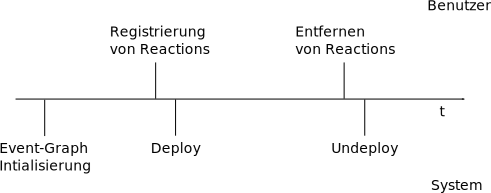
\includegraphics[width=0.7\textwidth]{graphics/EventNode-Lifecycle}
  \caption{Lifecycle eines EventNodes}
  \label{event_node_lifecycle}
\end{center}
\end{figure}


Es gibt, wie in Abb.\ref{interval_events_structure} zwei Klassen von
Intervall-Event-Nodes: BetweenEvents und ExecutionEvents. BetweenEvents sind vom
Auftreten des StartEvents bis zum Auftreten des ersten End-Events aktiv, wenn
eine Reaction registiert wurde. Das Execution-Event dient dazu, die Ausf"uhrung
einer Funktion zu protokollieren. Wenn das Execution-Event eine Funktion
"uberwachen soll, dann instrumentiert der Compiler die Funktion so, dass ein
Before-Event beim Betreten der Funktion und ein After-Event beim Verlassen der
Funktion ausgel"ost wird.

%\usepackage{graphics} is needed for \includegraphics
\begin{figure}[htp]
\begin{center}
  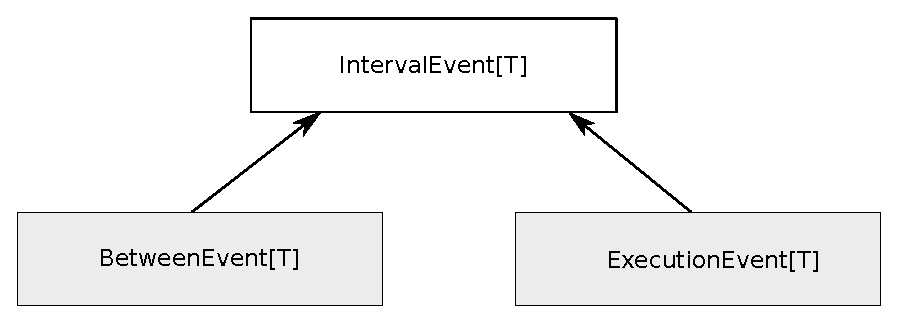
\includegraphics[width=0.5\textwidth]{graphics/interval_event_structure}
  \caption{Arten von Intervall-Events}
  \label{interval_events_structure}
\end{center}
\end{figure}

\subsection{Die Klasse IntervalEvent}
Die Klasse IntervalEvent stellt folgende Methoden zur Verfügung:

\begin{description}
\item{\bf before: } Das zum Interval zugehörige before-Ereignis wie oben definiert
\item{\bf after: } das after-Ereignis, wie oben definiert
\item{\bf value: } der Wert des Intervals, wie oben definiert. Zusätzlich wird via pull eine punktgenaue Abfrage ermöglicht,
Unterklassen sollten jedoch getValue stattdessen verwenden und Spezialfälle (Endpunkte des Intervals) gesondert behandeln
\item{\bf isActive: } den Wert des Active-Bits, wie oben definiert. Zusätzlich wird via pull der Anfangspunkt des Intervals eingeschlossen. Unterklassen sollten stattdessen active verwenden und den Spezialfall gesondert behandeln.
\item{\bf complement,\&\&,||,\textbackslash: } wie oben definiert
\item{\bf map(V => T):IntervalEvent[T] : } transformiert den Wert des Intervals
\item{\bf \&\&(\Interval{2},(V => Boolean)): } filtert Intervalle nach Werten
\end{description}

Zusätzlich stellt das Package scala.events die Methode \textit{Lazy(\Interval{})} zur Verfügung, die für die Deklaration von rekursiv oder zyklisch voneinander abhängigen Intervallen gebraucht werden kann. \textit{from} und \textit{to} erlauben die Definition von Intervallen, die nur einen Start- bzw. Endpunkt besitzen.

\subsection{Der Aufbau des Event-Graphen}
Mithilfe von Event-Nodes k"onnen mehrere Events zu komplexeren Events
zusammengefasst werden. So ist es beispielsweise m"oglich, alle Events einer
Filter-Bedingung zu unterziehen. Das resultierende Event wird nur dann
ausgel"ost, wenn ein zu filterndes Event auftritt dessen Filterbedingung zu
wahr auswertet. 

Der aus mehreren Event-Knoten bestehende Abhänigkeitsgraph soll nachfolgend als
Event-Graph bezeichnet werden. Ein Event-Graph besteht aus mindestens einem
Event-Node. Mehrere Event-Nodes können mit gerichteten Kanten verbunden sein. 
Es gibt zwei Arten von Kanten im Event-Graphen. Unbeschriftete Kanten zeigen 
die ``Flussrichtung'' von Events an. Kanten die mit pull() beschriftet sind, 
zeigen die zu prüfenden Abhängigkeiten bei einer Pull-Operation an. 
Except-Event-Knoten haben die Beschriftung ``$\backslash$''.

Wenn Intervall-Events im Eventgraph verwendet werden sollen, müssen die zum
Intervall gehörigen before- oder after-Events in den Eventgraph eingefügt
werden. Eine Liste der m"oglichen Filterfunktionen und die dazugeh"origen 
Definitionen findet sich im Kapitel \ref{definitions}.

\subsection{Auswertung des Eventgraphen}

Bei der Auswertung eines Event-Graphen gibt es zwei mögliche Vorgehensweisen.
Zum einen kann man Events sammeln, die bei einem Knoten des Event-Graphen
ankommen und dann weiterleiten, wenn gewisse Bedingungen erfüllt sind. Hierbei handelt es sich um
eine Push-basierte Implementierungen. Es werden n"amlich nur "Anderungen gepusht.

Beim Zweiten Ansatz werden keine Änderungen weitergeleitet. Stattdessen wird
der Event-Graph traversiert um herauszufinden, ob Änderungen passiert sind. Dieser
Ansatz wird nachfolgend als Pull-basiert bezeichnet.

Bei gleichem Resultat haben beide Implementierungen verschiedene Vor- und
Nachteile. Nachteilig beim Push-basierten Ansatz ist die relativ hohe Komplexität
der Implementierung wenn Knoten im Event-Graph einen Zustand aufweisen.
Dann ist es schwierig, ein deterministisches Verhalten sicherzustellen. Beim
Pull-basierten Ansatz stellt sich stattdessen die Frage, wie man den richtigen
Zeitpunkt f"ur einen Pull ermitteln kann. 

Die Implementierung im scala.events-Modul verwendet einen hybriden Ansatz um den
Event-Graphen auszuwerten. Die meisten Event-Knoten wurden Push-basiert
implementiert. Eine Ausnahme stellt der Except-Knoten dar. Mit einem solchen
Event-Knoten k"onnen verschiedene Events ausgeschlossen werden. Der Except-Zweig
des Event-Knotens wurde pull-basiert implementiert.

Betrachten wir nachfolgend zwei Beispiele um diese Vorgehensweise zu begr"unden:
\begin{eqnarray}
val \; e & = e1 \setminus (e2 || e3)\\
val \; e & = e1 \setminus (e1 || e3)
\end{eqnarray}

Der Event-Graph des Push-basierten Ansatzes ist in
Abb.\ref{push_based_event_graph} zu sehen. Wenn das Event e1 ausgelöst wird,
startet zunächst das Sammeln von Reactions im Knoten e1 und folgt den im
Diagramm eingezeichneten Kanten. 
 
Der Except-Event-Knoten speichert intern ob bereits ein Sammelvorgang über den
Except-Zweig durchgeführt wurde. Ist dies nicht der Fall, dann wird das Sammeln
in e forgesetzt und die Reaction auf das Event e wird gesammelt. 

Wenn allerdings schon eine Sammlung über den Except-Zweig erfolgte, dann
verhindert der Except-Knoten das Sammeln der Reactions von e.

Der in Abb.\ref{pull_based_event_graph} beschriebene Ansatz funktioniert
prinzipiell genauso. Allerdings wird im Except-Event-Node explizit der Pull-Vorgang ausgelöst um zu
prüfen, ob die Except-Bedingung gilt oder nicht. Der Except-Knoten speichert
dann keinen internen Zustand mehr.

Betrachten wir nun das Beispiel 2. Das Beispiel 2 ist praktisch von keiner
Bedeutung. Allerdings zeigt es gut die Probleme einer Push-basierten
Implementierung auf. 

Wenn der Event e1 ausgelöst wird, kann das Sammeln von Reactions nun mit zwei
Knoten starten wie man im Event-Graphen in Abb.
\ref{failing_push_based_event_graph} sehen kann. Möglicherweise werden die
Reactions vom Except-Knoten über den Or-Knoten zuerst gesammelt. Dann schaltet 
der Except-Knoten seinen internen Zustand um. Wenn anschließend die Sammlung
über  die zweite Kante von e1 erfolgt, hat sich der Zustand von Except bereits 
geändert, sodass keine Reaktionen von e gesammelt werden.

Wenn allerdings zunächst der Except-Knoten besucht wird, hat dieser seinen
internen Zustand noch nicht umgeschaltet. Dann werden die Reactions von e
gesammelt. Erst wenn später der Except-Knoten über den Or-Knoten besucht wird,
schaltet der Except-Knoten seinen Zustand um. Allerdings wurde dann schon die
Reaction von e gesammelt. Daher muss, wenn der Except-Knoten über den
Except-Zweig erreicht wird, die Liste mit Reactions gelöscht werden. Das hier
genannte Beispiel 2 würde dann korrekt arbeiten. Allerdings lassen sich durch
kompliziertere Beispiele Zustände erzeugen, bei dem das korrekte Sammeln von
Events scheitert\footnote{Ein Beispiel hierfür ist ein Event-Graph bei dem sich
über dem Except-Knoten ein And-Knoten befindet}.

Der Pull-basierte Ansatz ist in Abb. \ref{working_pull_based_event_graph} zu
sehen. Hier gibt es in e1 nur einen Weg, die Sammlung der Reactions zu
beginnen\footnote{Natürlich gibt es auch hier wieder zwei Wege von e1 zum
Except-Knoten. Allerdings stellt der Weg über den Or-Knoten eine Sackgasse
dar. Sammler die den Except-Knoten über diesen Weg erreichen, werden ignoriert
und sammeln keine Reactions ein.}. Wenn der Reaction-Sammler nun im
Except-Event-Knoten angelangt, wird eine Pull-Operation auf den Except-Zweig ausgeführt. Dabei  wird
festgestellt, dass der auslösende Event ebenfalls über die Except-Kante beim 
Except-Knoten ankommt. Daher werden keine Reactions von e gesammelt.


 


%\usepackage{graphics} is needed for \includegraphics
\begin{figure}[htp]
\centering
\subfigure[Push basierter Event-Gaph] {
  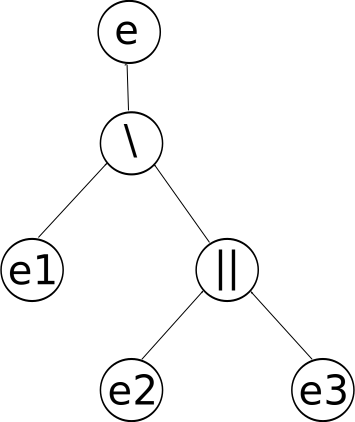
\includegraphics[width=0.3\textwidth]{graphics/event_node_except_push}
  \label{push_based_event_graph}
}
\subfigure[Push/Pull basierter Event-Graph] {
  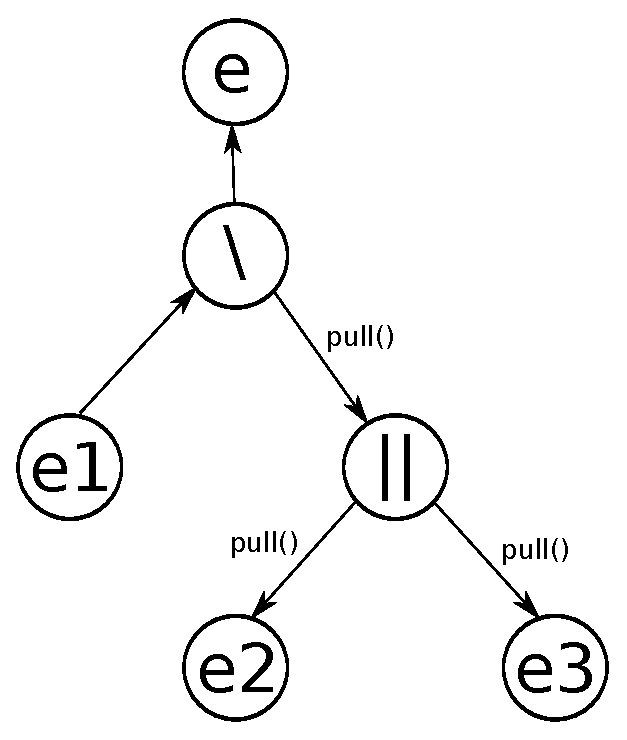
\includegraphics[width=0.3\textwidth]{graphics/event_node_except_pull}
  \label{pull_based_event_graph}
}
\caption{Event-Graphen f"ur das Beispiel 1}
\end{figure}

\begin{figure}[htp]
\centering
\subfigure[Push basierter Event-Gaph] {
  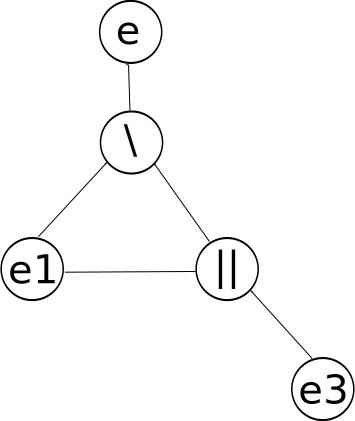
\includegraphics[width=0.3\textwidth]{graphics/event_node_except2_push}
  \label{failing_push_based_event_graph}
}
\subfigure[Push/Pull basierter Event-Graph] {
  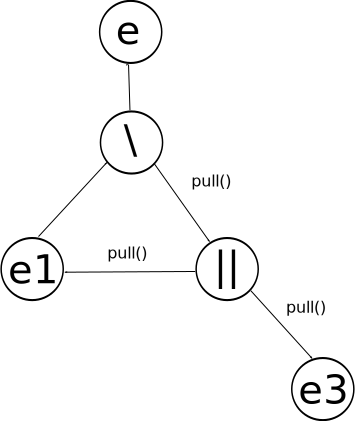
\includegraphics[width=0.3\textwidth]{graphics/event_node_except2_pull}
  \label{working_pull_based_event_graph}
}
\caption{Event-Graphen f"ur das Beispiel 2}
\end{figure}


